\documentclass[11pt]{article}

% --------------------
% Packages
% --------------------
\usepackage[utf8]{inputenc}
\usepackage[T1]{fontenc}
\usepackage{lmodern}
\usepackage{geometry}
\geometry{margin=1in}
\usepackage{setspace}
\onehalfspacing
\usepackage{hyperref}
\usepackage{enumitem}
\usepackage{booktabs}
\usepackage{tikz}
\usetikzlibrary{positioning}

% --------------------
% Metadata
% --------------------
\title{\textbf{Intent-Oriented Programming}\\
\large A Deterministic Paradigm for AI-Driven Software Development}
\author{Serkan Yersen}
\date{}

\begin{document}
\maketitle

\vspace{1em}

% ============================================================
\section{Introduction}

AI-assisted development has dramatically increased the speed at which software can be produced. However, this speed has come at the cost of predictability, architectural integrity, and long-term maintainability. Modern AI coding tools operate primarily as autonomous agents: heuristic systems that infer intent from loosely specified prompts and directly modify production code.

For professional software engineering organizations, this model introduces systemic risk. Engineering is not merely the act of producing code; it is the practice of making durable, auditable, and reversible decisions under constraints. When AI systems are treated as creative collaborators rather than deterministic tools, they undermine the very properties—control, reviewability, and intent preservation—that engineering teams depend on.

Intent-Oriented Programming (IOP) proposes a fundamentally different approach. Instead of asking AI systems to infer intent from code or prompts, IOP makes intent the primary artifact. Code becomes a derived output, generated and maintained to satisfy explicit, human-authored intent specifications.

This shift reframes AI from an autonomous decision-maker into a constrained execution mechanism. The result is a development paradigm that preserves AI-driven velocity while restoring determinism, safety, and long-term architectural coherence.

% ============================================================
\section{The Core Problem: AI as an Unbounded Collaborator}

The dominant AI-assisted development model today follows a simple pattern:

\begin{center}
\emph{Prompt $\rightarrow$ AI Agent $\rightarrow$ Codebase}
\end{center}

This model fails in professional environments for three structural reasons.

\subsection{Monolithic and Opaque Changes}

Autonomous agents frequently produce large, monolithic diffs that are difficult to review and reason about. The reviewer is forced to validate implementation details rather than intent, turning code review into forensic analysis.

\subsection{Implicit and Unstable Decisions}

AI agents make numerous unstated choices—libraries, patterns, abstractions—without recording them as explicit decisions. These choices are unstable across runs, leading to architectural drift and brittle systems.

\subsection{Loss of Conceptual Integrity}

Even when code is functionally correct, its underlying rationale is often opaque. Over time, teams inherit codebases where intent must be reverse-engineered from implementation, significantly increasing maintenance cost.

These are not incidental flaws. They are the direct result of allowing AI systems to operate beyond well-defined authority boundaries.

% ============================================================
\section{The Fundamental Shift: From Code to Intent}

Intent-Oriented Programming resolves these issues by changing what developers author.

\subsection{Intent as the Source of Truth}

In IOP, developers do not author code directly. Instead, they author structured, human-readable intent files that declaratively specify:

\begin{itemize}
  \item Purpose
  \item Behavior
  \item Constraints
  \item Architectural relationships
\end{itemize}

These intent files are the \textbf{single canonical source of truth}. Code is a derived artifact, regenerated as needed to satisfy the declared intent.

\subsection{Redefining the Role of AI}

Under IOP:

\begin{itemize}
  \item AI does not interpret high-level goals.
  \item AI does not decide scope.
  \item AI does not make architectural choices.
\end{itemize}

AI systems operate solely as constrained implementation engines executing a pre-approved plan.

This distinction is critical. IOP does not attempt to make AI “smarter.” It makes AI \emph{irrelevant to decision-making}.

% ============================================================
\section{System Boundary and Trust Model}

IOP explicitly defines authority boundaries within the system.

\begin{center}
\begin{tabular}{ll}
\toprule
Component & Authority \\
\midrule
Human-authored intent & Defines meaning and scope \\
Orchestrator & Computes diffs and plans deterministically \\
AI agents & Execute constrained implementation tasks \\
\bottomrule
\end{tabular}
\end{center}

Only the first two components are trusted to make architectural decisions. AI agents are interchangeable and replaceable.

This trust model eliminates silent scope expansion and ensures all meaningful change flows through a deterministic pipeline.

% ============================================================
\section{The Orchestrator: A Deterministic Compiler for Intent}

The Orchestrator is a traditional, non-LLM compiler that operates over intent specifications.

\subsection{Compilation Pipeline}

\begin{center}
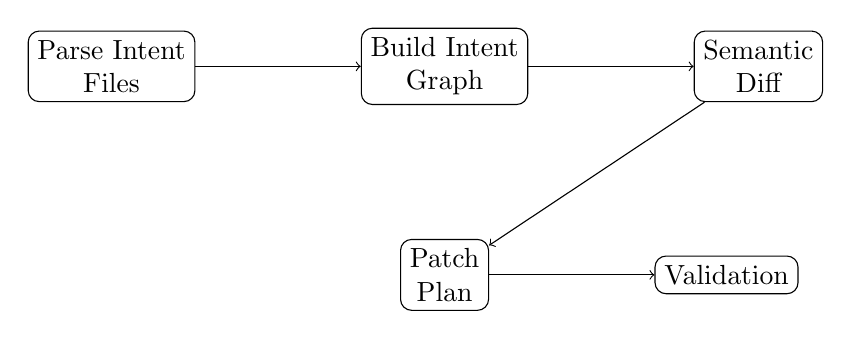
\begin{tikzpicture}[
    node distance=1.7cm and 2.1cm,
    every node/.style={draw, rectangle, rounded corners, align=center}
]
  % First row
  \node (parse)    {Parse Intent\\Files};
  \node (graph)    [right=of parse] {Build Intent\\Graph};
  \node (diff)     [right=of graph] {Semantic\\Diff};

  % Second row
  \node (plan)     [below=of graph] {Patch\\Plan};
  \node (validate) [right=of plan] {Validation};

  % Arrows
  \draw[->] (parse) -- (graph);
  \draw[->] (graph) -- (diff);
  \draw[->] (diff) -- (plan);
  \draw[->] (plan) -- (validate);
\end{tikzpicture}
\end{center}
\subsection{Semantic Diffing}

Unlike textual diffs, semantic diffs operate on intent structure:

\begin{quote}
\texttt{MODIFY\_BLOCK(component.todo\_list.v1::interaction.drag\_drop)}
\end{quote}

This representation captures meaning, not syntax, enabling precise and minimal change plans.

\subsection{Patch Plan Generation}

The Orchestrator produces a stable, reviewable Patch Plan consisting of ordered, scoped tasks. No code is modified until this plan is explicitly approved by a human.

% ============================================================
\section{Intent as a First-Class Architectural Primitive}

\subsection{Intent Structure}

An intent consists of:

\begin{itemize}
  \item \textbf{Header}: stable identity, kind, version
  \item \textbf{References}: declarative dependencies (\texttt{uses}, \texttt{renders})
  \item \textbf{Atomic Blocks}: ID-addressed intent statements
\end{itemize}

Atomic blocks are the smallest diffable unit, allowing changes to be localized and auditable.

\subsection{The Intent Graph}

All intents form a closed-world graph representing the complete system architecture. This graph is analyzable before any code is generated, enabling impact analysis and invariant enforcement.

% ============================================================
\section{Change as a Safe, Auditable Process}

IOP decomposes change into two explicit steps:

\subsection{Step 1: Declare Semantic Change}

Developers modify intent, not code. The change is expressed in terms of meaning.

\subsection{Step 2: Review the Execution Plan}

The Orchestrator generates a task-level plan with explicit scope and constraints. This plan is reviewed and approved before execution.

This model eliminates surprise, scope creep, and unintended side effects.

% ============================================================
\section{Lifecycle Management and Long-Term Evolution}

\subsection{Refactoring as Planned Migration}

Large refactors are expressed as Migration Intents—multi-step transformations with enforced invariants. Refactoring becomes a controlled process, not a risky event.

\subsection{Safe Decommissioning}

Intents move through a managed lifecycle:

\begin{center}
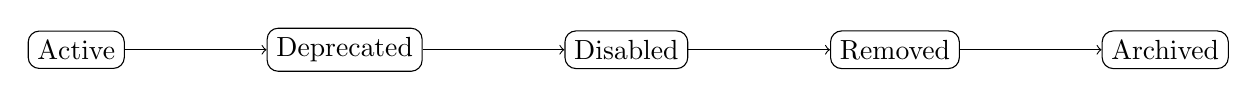
\begin{tikzpicture}[node distance=1.8cm, every node/.style={draw, rectangle, rounded corners}]
\node (a) {Active};
\node (d) [right=of a] {Deprecated};
\node (di) [right=of d] {Disabled};
\node (r) [right=of di] {Removed};
\node (ar) [right=of r] {Archived};

\draw[->] (a) -- (d);
\draw[->] (d) -- (di);
\draw[->] (di) -- (r);
\draw[->] (r) -- (ar);
\end{tikzpicture}
\end{center}

This enables automated, safe removal of dead code without breaking dependencies.

% ============================================================
\section{Adoption and Ejection}

\subsection{Incremental Adoption}

IOP supports brownfield projects via intentification: reverse-engineering existing code into intent while leaving the remainder untouched.

\subsection{Zero Lock-In Guarantee}

IOP-generated code has no runtime dependencies. The system can be fully removed at any time, leaving a clean, conventional codebase.

% ============================================================
\section{Failure Modes and Explicit Non-Goals}

IOP makes the following guarantees:

\begin{itemize}
  \item Deterministic plans from identical intent
  \item No silent scope expansion
  \item Human approval of all changes
\end{itemize}

IOP explicitly does not guarantee:

\begin{itemize}
  \item Optimal implementations
  \item Semantic correctness beyond declared intent
  \item Elimination of all bugs
\end{itemize}

These boundaries are intentional and necessary.

% ============================================================
\section{Conclusion}

Intent-Oriented Programming restores engineering discipline to AI-driven development by enforcing a strict separation between intent and implementation. By elevating intent to the primary artifact and constraining AI to deterministic execution, IOP enables teams to scale software systems without sacrificing safety, clarity, or control.

The paradigm shift is simple but profound: humans author meaning; machines execute tactics. Everything else follows.

\end{document}
